\chapter{Implementación del sistema de reconocimiento de gestos propuesto}\label{capit:cap4}
\vspace{-2.0325ex}%
\noindent
\rule{\textwidth}{0.5pt}
\vspace{-5.5ex}% 
\newcommand{\pushline}{\Indp}% Indent puede ir o no :p

En este cap\'itulo se describe los detalles de implementación del sistema.  

\section{Adquisición de los datos}\label{sec:AdquisicionDatos}

En esta etapa se capturan los datos que son la entrada del sistema. Los datos provienen de los sensores de profundidad de dos dispositivos Kinect, estos se encuentran ubicados uno frente al  usuario y otro al lado  izquierdo como se muestra en la figura \ref{fig:SetupSystem}.

\begin{figure}[!h]
\begin{center}
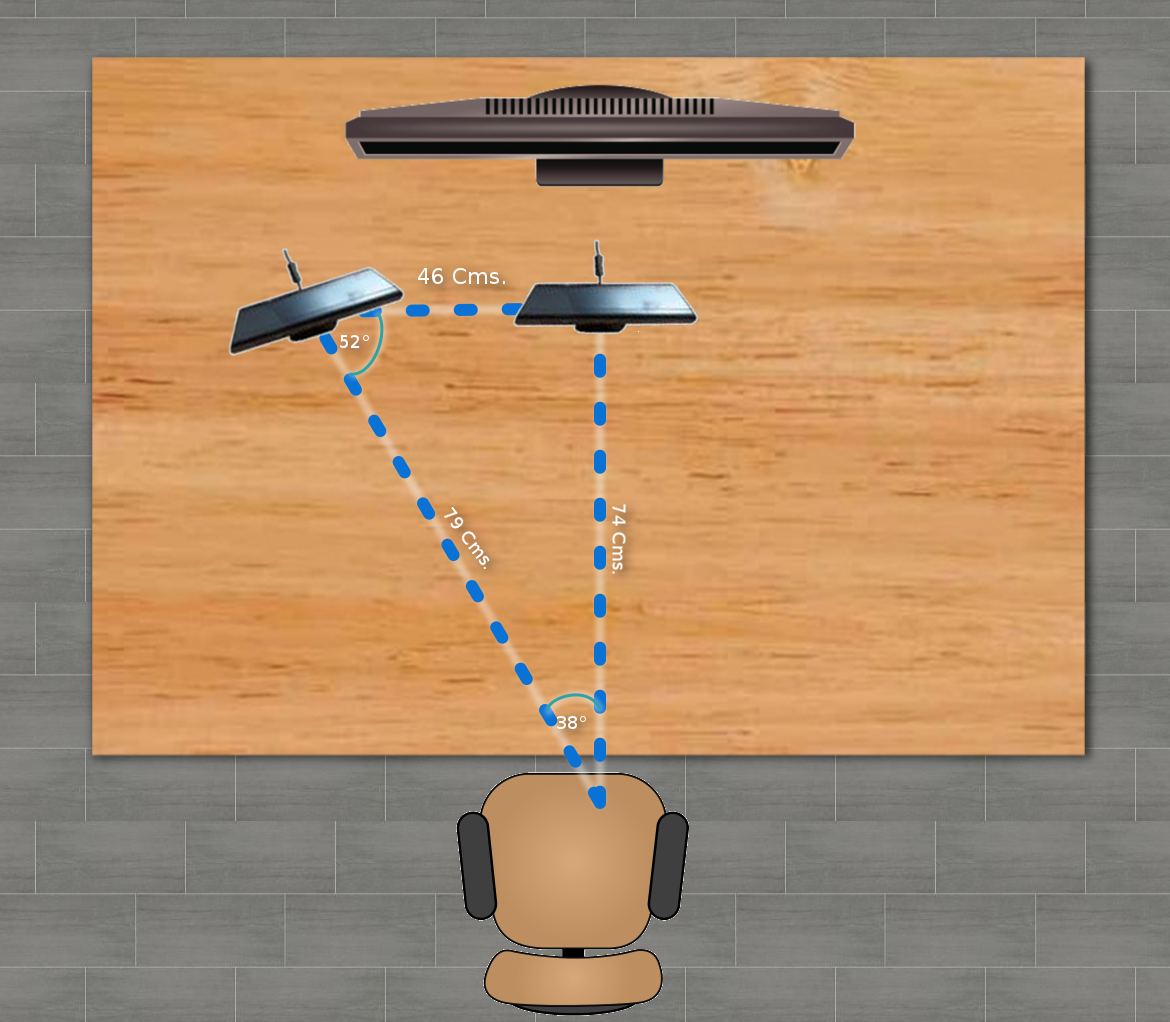
\includegraphics[scale=.2]{./Figures/system.png}
\end{center}
\caption{Configuración del sistema de reconocimiento de gestos con las manos}
\label{fig:SetupSystem}
\end{figure} 
 
una vez que le flujo de datos de los sensores de profundidad es capturado este es representado como una imagen en escala de grises de $8$ bits de $640$ p\'ixeles de ancho por $480$ p\'ixeles de largo. En las imágenes se puede apreciar detalles pequeños, es decir cambios en la profundidad de hasta $1$  $mm$ esto debido a que la escala de grises inicia cada $26$  $cm$. %creo que no se entiende bien, explicar un poco mejor.  
En la siguiente imagen se puede apreciar un ejemplo de las imágenes de profundidad. \ref{fig:ImagenCapturada}

\begin{figure}[!h]
\begin{center}
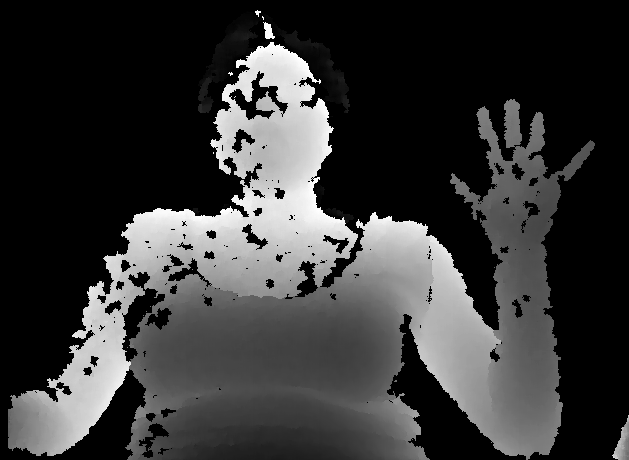
\includegraphics[scale=.5]{./Figures/166.png}
\end{center}
\caption{Representación de los datos capturados por los Kinect}
\label{fig:ImagenCapturada}
\end{figure}  

Debido a la naturaleza del funcionamiento del Kinect, las imágenes obtenidas contiene ruido del tipo (poner), el cual nos da una imagen como la figura  , el ruido  es reducido usando un filtros de mediana este es aplicado en toda la imagen en una ventada de tama\~no $13$. La imagen resultante $S(x,y)$ es como la que se muestra en la figura \ref{fig:ImagenCapturada}

\begin{figure}[!h]
\begin{center}
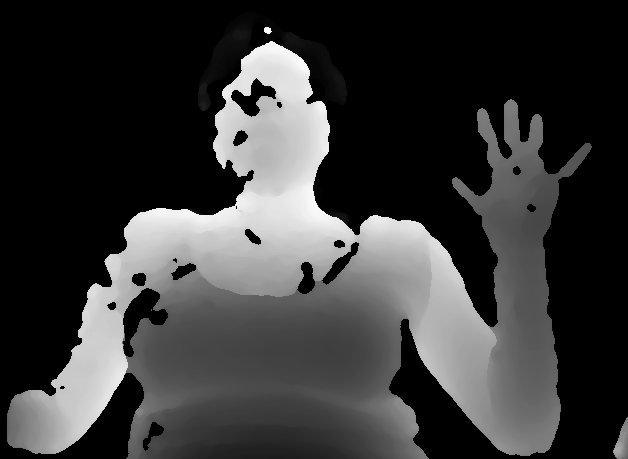
\includegraphics[scale=.5]{./Figures/166_W13.png}
\end{center}
\caption{Representación de los datos capturados por los Kinect}
\label{fig:ImagenCapturadaNoNoise}
\end{figure}  
  

%\begin{center}[a]
%\begin{tabular}{ c c c }
% cell1 & cell2 & cell3 \\ 
% cell4 & cell5 & cell6 \\  
% cell7 & cell8 & cell9    
%\end{tabular}
%\end{center}
%
%\begin{center}[b]
%\begin{tabular}{ |c|c|c| } 
% \hline
% cell1 & cell2 & cell3 \\ 
% cell4 & cell5 & cell6 \\ 
% cell7 & cell8 & cell9 \\ 
% \hline
%\end{tabular}
%\end{center}
%
%\begin{center}[c]
% \begin{tabular}{||c c c c||} 
% \hline
% Col1 & Col2 & Col2 & Col3 \\ [0.5ex] 
% \hline\hline
% 1 & 6 & 87837 & 787 \\ 
% \hline
% 2 & 7 & 78 & 5415 \\
% \hline
% 3 & 545 & 778 & 7507 \\
% \hline
% 4 & 545 & 18744 & 7560 \\
% \hline
% 5 & 88 & 788 & 6344 \\ [1ex] 
% \hline
%\end{tabular}
%\end{center}
%
%\begin{center}[d]
%\begin{tabular}{ | b{5cm} | m{2cm}| m{2cm} | } 
%\hline
%The aligning options are m for middle, p for top and b for bottom.& cell2 & cell3 \\ 
%\hline
%cell1 dummy text dummy text dummy text & cell5 & cell6 \\ 
%\hline
%cell7 & cell8 & cell9 \\ 
%\hline
%\end{tabular}
%\end{center}
%
%\begin{center}[e]
%\begin{tabular}{ |p{3cm}||p{3cm}|p{3cm}|p{3cm}|  }
% \hline
% \multicolumn{4}{|c|}{Country List} \\
% \hline
% Country Name     or Area Name& ISO ALPHA 2 Code &ISO ALPHA 3 Code&ISO numeric Code\\
% \hline
% Afghanistan   & AF    &AFG&   004\\
% Aland Islands&   AX  & ALA   &248\\
% Albania &AL & ALB&  008\\
% Algeria    &DZ & DZA&  012\\
% American Samoa&   AS  & ASM&016\\
% Andorra& AD  & AND   &020\\
% Angola& AO  & AGO&024\\
% \hline
%\end{tabular}
%\end{center}
%\begin{center}[f]
%\begin{tabular}{ |c|c|c|c| } 
%\hline
%col1 & col2 & col3 \\
%\hline
%\multirow{3}{4em}{Multiple row} & cell2 & cell3 \\ 
%& cell5 & cell6 \\ 
%& cell8 & cell9 \\ 
%\hline
%\end{tabular}
%\end{center}

\section{Detección}\label{sec:DeteccionSystem} 

En esta etapa del sistema el objetivo es localizar y segmentar la mano para extraer las características necesarias para el reconocimiento. 
En este trabajo se utiliza el algoritmo de detección de objetos desarrollado por \citep{Viola2001}, como se mostró en el cap\'itulo \ref{capit:cap2} sección \ref{sec:ViolaJones}, el algoritmo  clasifica las imágenes basándose en el valor de características. 


La selección de las características se llev\'o acabo por medio del algoritmo AdaBoost; la implementaci\'on se realiz\'o utilizando el software OpenCV Haar training classifier \footnote{https://github.com/mrnugget/opencv-haar-classifier-training}. Se entren\'o con $1000$ imágenes positivas (imágenes de profundidad de la mano), y $2000$ negativas, (imágenes de fondo a distintas profundidades). Las imágenes positivas fueron generadas de $100$ imágenes de la mano usando el software Create Samples \footnote{http://note.sonots.com/SciSoftware/haartraining.html}. Todas las imágenes usadas fueron tomadas de nuestra base de  datos \footnote{https://github.com/americamm}.

Nuestra base de datos contiene gran cantidad de imágenes de profundidad. Imágenes de fondo y de mano, estas fueron tomadas a una distancia de entre $60$ $cm$ y $200$ $cm$. Las imágenes de profundidad de la mano fueron tomadas de $6$ personas distintas con tres distintas poses: palma abierta con dedos abiertos, palma abierta con dedos juntos y finalmente el pu\~no, como se muestra en la figura \ref{fig:ImagenesPoses}. Las imágenes de fondo fueron tomadas de distintos escenarios como se muestra en la figura \ref{fig:ImagenFondo}. El programa para la captura de las imágenes puede ser encontrado en github \footnote{https://github.com/americamm}.  

\begin{figure}[h!]
\begin{center}
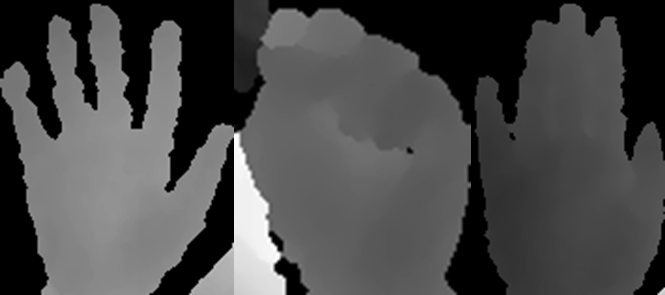
\includegraphics[scale=.5]{./Figures/TrainingImages.png}
\end{center}
\caption{Imágenes de la mano de nuestra base de datos}
\label{fig:ImagenesPoses}
\end{figure}  

\begin{figure}[h!]
\begin{center}
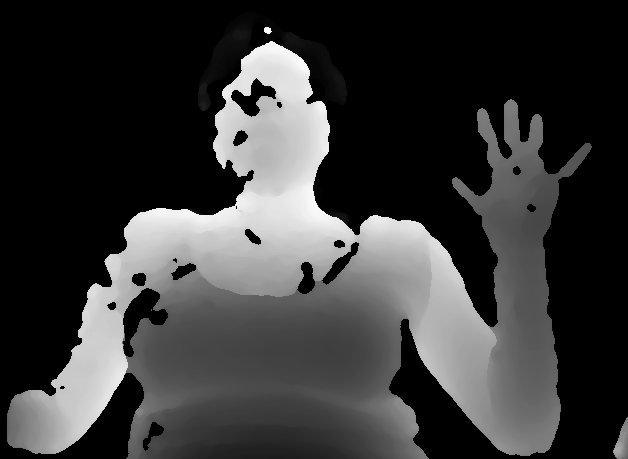
\includegraphics[scale=.5]{./Figures/166_W13.png}
\end{center}
\caption{Imágenes del fondo de nuestra base de datos}
\label{fig:ImagenFondo}
\end{figure}  

Para localizar la mano en cada cuadro proveniente de los Kinect, una ventana de tamaño $kahkjgv$ se desliza por la imagen, una vez que la mano se localiza la región de interés $ROI(x,y)$ es seleccionada alrededor de la mano, como se puede ver en la figura \ref{fig:Roi}.

\begin{figure}[h!]
\begin{center}
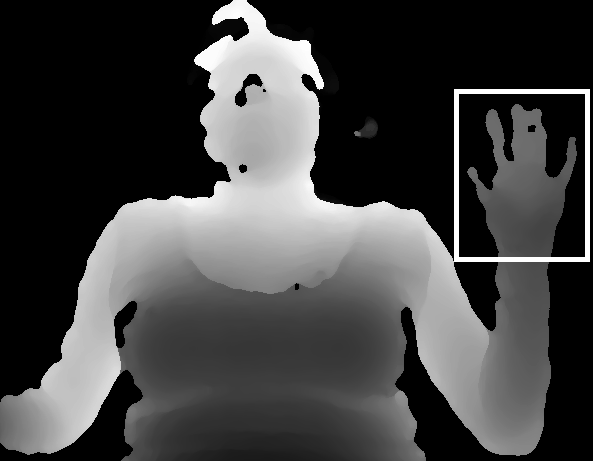
\includegraphics[scale=.5]{./Figures/roi.png}
\end{center}
\caption{Mano seleccionada}
\label{fig:Roi}
\end{figure}  

Ya que se tiene localizada el área donde se encuentra la mano, el siguiente paso es segmentar la mano del ROI. La segmentación se realiza calculando los contornos existentes en la ROI y se toma el contorno más grande como el contorno de la mano, antes de calcular el contorno se realizan una serie de procesamientos al ROI para eliminar ruido y que el cálculo del contorno sea más preciso.    

El primer procesamiento que se aplica al ROI, son las operaciones morfológicas de apertura y cerradura, en ese orden. Se utilizan para eliminar uniones pequeños que existen en la imagen como el que se muestra \ref{fig:RuidoUnion} o unir pequeños hoyos que existen en la imagen, como los que se encuentran en la figura \ref{fig:RuidoHoyo}.\\
La operaciones utilizan un elemento estructural rectangular; para la operación de apertura el tamaño del elemento $3 \, x \, 7$ pixeles; para la cerradura se aplic\'o con un tamaño  $7 \, x \, 7$ pixeles. 

\begin{figure}[h!]
\begin{center}
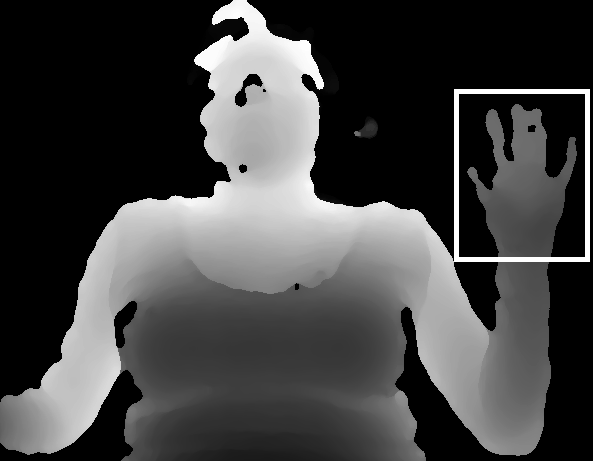
\includegraphics[scale=.5]{./Figures/roi.png}
\end{center}
\caption{ROI que muestra una unión entre los dedos}
\label{fig:RuidoUnion}
\end{figure}   

\begin{figure}[h!]
\begin{center}
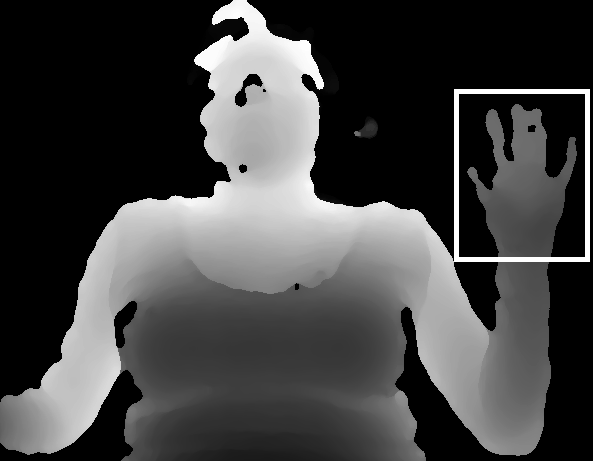
\includegraphics[scale=.5]{./Figures/roi.png}
\end{center}
\caption{ROI donde se aprecio un hoyo en la mano}
\label{fig:RuidoHoyo}
\end{figure}  


El resultado de estas operaciones es mejorar la región de interés. Las imágenes siguientes muestran el resultado de aplicar las operaciones apertura y cerradura al ROI. 

\begin{figure}[!h]
\begin{center}
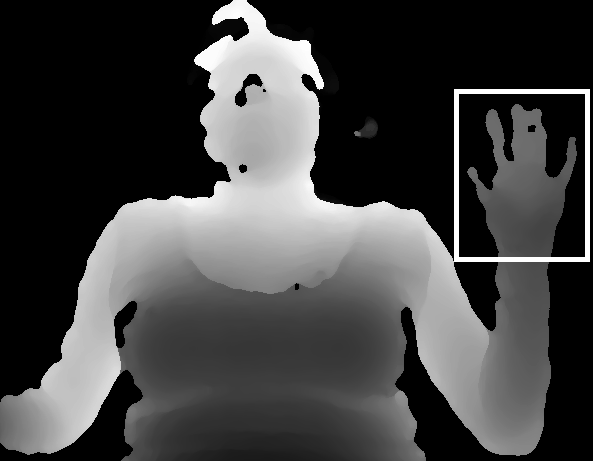
\includegraphics[scale=.5]{./Figures/roi.png}
\end{center}
\caption{Apertura y cerradura}
\label{fig:ImagenOpenClose}
\end{figure}  

Una vez aplicadas las operaciones el siguiente paso es binarizar la región de interés, se lleva acabo aplicando el algoritmo desarrollado por \citep{Niblack1985}, se decidió usar este método debido a la naturaleza de la imagen. Los parámetros que fueron usados fueron $k=0.5$ y una ventana de $3x3$ p\'ixeles. La imagen siguiente es una imagen binarizada. 

\begin{figure}[!h]
\begin{center}
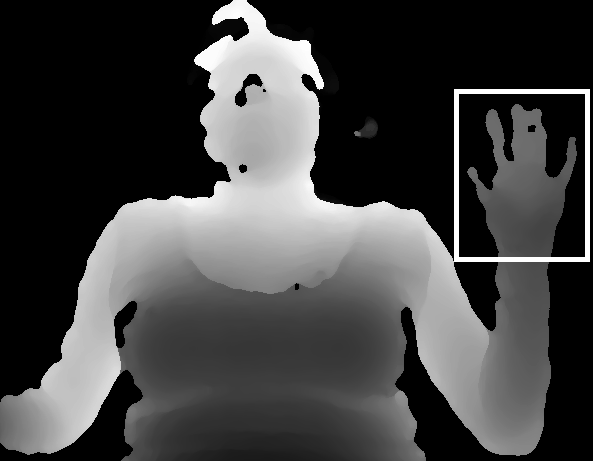
\includegraphics[scale=.5]{./Figures/roi.png}
\end{center}
\caption{Binarización de ROI}
\label{fig:BinarizationRoi}
\end{figure}
 
%\begin{table}
%\footnotesize
%\centering
%\caption{Mauris et imperdiet     tortor. Maecenas consectetur lacus elit, dignissim eleifend dolor  ornare ut. Aenean euismod porta nisi, et volutpat ex laoreet sit amet. Sed ac elit vestibulum neque ultrices feugiat}
%\label{tab:recopilacionDeCuestionarios}
%%\rotatebox{90}{
%\begin{tabular}{m{0.2cm}m{2.5cm}m{2.5cm}m{2.5cm}m{2.5cm}m{2.5cm}}
%\hline\noalign{\smallskip}
% & \textbf{FFS} & \textbf{SOFA} & \textbf{FQ} & \textbf{CIS20R} & \textbf{FACIT}
%\\ \noalign{\smallskip}
%\hline
%\noalign{\smallskip}
%1	&	TAF	&	TAF	&	PF	&	PF	&	PF\\
%2	&	TAF	&	CM	&	CS	&	EE	&	PF\\
%3	&	PF	&	TAF	&	CS	&	CM	&	EE\\
%\hline
%\end{tabular}
%%}
%\end{table}

Una vez que la ROI es binarizada, el siguiente paso es encontrar los contornos existentes dentro de esta. Los contornos se calcularon utilizando el algoritmo de $blabla$ con tales parámetros.  

Ya que le contorno de la mano es identificado, se calcula el casco convexo de la mano y posteriormente los defectos de convexidad 

\section{Extracci\'on de caracter\'isticas}\label{sec:ExtraccionCaracteristicasSystem}

Para la extracción de características se utilizan los algoritmos de casco convexo y el de defectos de convexidad, la figura muestra la mano con el casco convexo y sus defectos. 

\begin{figure}[!h]
\begin{center}
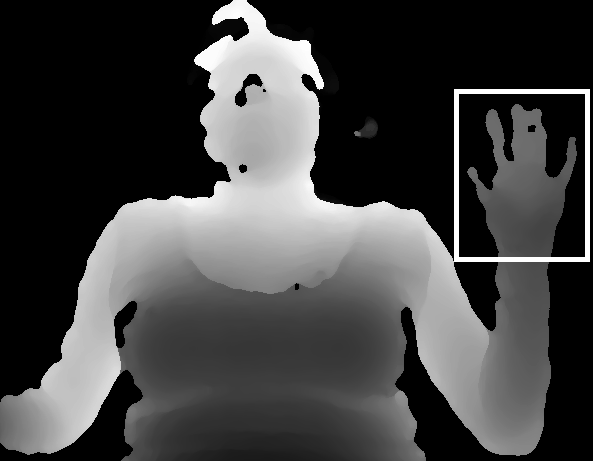
\includegraphics[scale=.5]{./Figures/roi.png}
\end{center}
\caption{En esta dibujado el casco convexo los punto en son los defectos de convexidad}
\label{fig:Convex&Defects}
\end{figure}


Una vez aplicados estos dos algoritmos se pueden calcular el número de dedos y las puntas de estos que son fundamentales para calcular las demás características. Enseguida se describe el algoritmo () para calcular el numero de dedos. 
Sea $CD={cd_1, cd_2, \cdots, cd_n}$ los defectos de convexidad de un conjunto casco convexo. Cada defecto esta compuesto de tres elementos $s_i(x,y),d_i(x,y),e_i(x,y) \in cd_i$. $\delta_i$ es la distancia de $d_i(x,y)$ a la orilla del casco convexo.  

\begin{algorithm}
\begin{algorithmic}[1]

\REQUIRE $d_i$
\ENSURE Número de dedos, $Nf$.  

\FOR{$i=1$ hasta $n$}  
	\STATE $minDist=20$, $maxAng=60$, $antecesor=0$, $sucesor=0$. 	
	
	\IF{$\delta_i < minDepth$ } 
	\STATE continuar
	\ENDIF 
	
	\IF{i=0} 
	\STATE $antecesor=n-1$
	\ELSE
	\STATE $antecesor=i-1$
	\ENDIF 

	\IF{i=n-1} 
	\STATE $sucesor=0$
	\ELSE
	\STATE $sucesor=i+1$
	\ENDIF   
	
	\STATE Calcular el $angulo$ entre $s_{antecesor}(x,y)$ y $s_{sucesor}(x,y)$
	
	\IF{$angulo \geqslant maxAng$}
	\RETURN \FALSE
	\ENDIF  
	
	\STATE $Nf=Nf+1$.

\ENDFOR 

\end{algorithmic}
\end{algorithm}


Calculo del $angulo$

$$ \alpha_{f_j} = \tan^{-1}{ \bigg| \frac{m_{j+1}-m_j}{1+m{j+1}m_j} \bigg|}$$

$$ \theta_{f_j} = \tan^{-1} | {m_j} - 90^\circ |$$


 

%\begin{equation} \label{eq:demandaOxigeno_simple}
%\begin{split} 
%& K = R + H + V \\ 
%& R = \textrm{consumo de oxígeno} \times kg^{-1} \times min^{-1}\\ 
%& H = \textrm{constante horizontal} \times \textrm{velocidad de desplazamiento}\\ 
%& V = \textrm{constante vertical} \times \textrm{velocidad de desplazamiento}\\ 
%\end{split} 
%\end{equation} 
%
%\begin{figure}\label{eq:testing}
%\[ e = m c^2 \]
%\caption{A $ \dfrac{3}{2} $ famous equation, where $ e = m c^2  $ represent $ e = m c^2  $ energy something and $  A_{d} = -g - \frac{\sum F}{mass} $  another $\protect\pi=\protect\varpi + \protect\xi$ thing. }
%\end{figure}


Las características se guardan en un vector de características de dimensión $26$.

\section{Reconocimiento}\label{sec:ReconocimientoSystem}

Es la etapa final del reconocimiento,es donde finalmente el gesto puede ser interpretado por la computadora.   
El reconocimiento de los gestos estáticos se lleva acabo usando el algoritmo de clasificación de SVM. 




%\subsection{Extracción de parámetros}
%Ecuación \ref{eq:gravedad}. 
%
%\begin{equation} \label{eq:gravedad}
%A_{d} = -g - \frac{\sum F}{mass}
%\end{equation} 

%Donde $A_{d}$ representan la aceleración que se aplica a un dispositivo, $g$ la constante de gravedad de 9.81 m/$s^{2}$, y $\sum F$ las fuerzas que se aplican al propia sensor.

%Text  \ref{eq:demandaOxigeno_personalizada} and more $O_{2}$ text:
%
%\begin{equation} \label{eq:demandaOxigeno_personalizada}
%\begin{split} 
%& K = R + H + V \\ 
%& R = 3.5 - (0.0367 \times BMI) - (0.0038 \times age) + (0.1790 \times gender)\\
%& H = 0.1 \times \textrm{velocidad de desplazamiento}\\ 
%& V = 1.8 \times \textrm{velocidad de desplazamiento}\\ 
%\end{split} 
%\end{equation} 
%
%Donde $1 + 2$ representan el consumo de $O_{2}$ en reposo personalizado al usuario $(ml \times kg^{-1} \times min^{-1})$ \citep{Barstow:1991}, $H$ el componente horizontal relativo a la velocidad de desplazamiento (m/min), $V$ el componente vertical relativo a la velocidad (m/min) y pendiente de desplazamiento (\%).
%
%\begin{description}
%  \item[Velocidad:] \hfill \\
%  	Para obtener la velocidad de desplazamiento se utiliza el número de pasos realizados por el usuario como se muestra a continuación (Ecuación \ref{eq:velocidad}).
%  
%\begin{equation} \label{eq:velocidad}
%  S_{k} = D_{k}/W \hspace{10 mm} 
%  D_{k} = ST_{k} \times SL \hspace{10 mm}
%  SL = D_{total}/ST_{total} 
%\end{equation}
%\end{description}
	
\newpage
%%=====================================================

